\documentclass[12pt]{article}
\bibliographystyle{IEEEtran}
\usepackage{graphicx,fancyhdr,parskip}
\setlength{\parskip}{.5cm plus4mm minus3mm}
\usepackage[margin=1in]{geometry}
\usepackage[colorlinks]{hyperref}
\usepackage{color}
\definecolor{darkblue}{rgb}{0,0,0.5}
\hypersetup{
    colorlinks=true,
    urlcolor=blue,
    citecolor=black,
    linkcolor=darkblue
}
\usepackage[nonumberlist]{glossaries}
\renewcommand{\glossarysection}[2][]{}
\makeglossaries
\usepackage{makeidx}
\makeindex
\makeatletter
  \renewcommand\@seccntformat[1]{\csname the#1\endcsname.\quad}
\makeatother
%\def\thesection {\Alph{section}}
%\def\thesubsection {\alph{subsection}}
%\def\thesubsubsection {\arabic{subsubsection}}
\usepackage{titlesec}
\titlespacing{\subsection}{2em}{0pt}{0pt}

\pagestyle{fancy}
\fancyhead[LO]{SiQuoia cost estimates (Team Q06)}
\fancyfoot[RO]{\copy SQ06 \year}

\hyphenation{op-tical net-works semi-conduc-tor}

\begin{document}
\title{CS160 - SiQuoia Cost Estimates \\ {\normalsize Version 2}}

%\author{ Ryan Alcoran \and Joe Lee \and Shivalik Narad \and Nam Phan
%  \and Swapna Vemparala \and Amber Wong }
\author{{\Large Team Q06}}

\begin{titlepage}
\maketitle

{\bf Project Team}
\begin{center}
\begin{tabular}{p{4cm} l}
{\bf Names}         & {\bf Roles} \\[.5em]
Joe Lee             & Business Manager \\[1em]
Swapna Vemparala    & Project Manager \\[1em]
Shivalik Narad      & Development Manager 1 \\[1em]
Nam Phan            & Development Manager 2 \\[1em]
Amber Wong          & Risk Manager \\[1em]
Ryan Alcoran        & Test Manager
\end{tabular}
\end{center}

{\bf Project Team}
\begin{center}
\begin{tabular}{|l|l|l|}
\hline
{\bf Date}      & {\bf Reasons for change}  & {\bf Version} \\
\hline
09/14/2013      & Initial creation          & v1 \\
\hline
11/20/2013      & Update cost estimates.    & v2 \\
\hline
\end{tabular}
\end{center}

\end{titlepage}

\section{Introduction}

\subsection{Purpose}
The cost estimation document contains detailed estimates of the costs
incurred for implementing SiQuoia based on the requirements specified
by the client. It is intended for all stakeholders of the SiQuoia
system.

\subsection{Scope}
This document provides a projected cost analysis of the SiQuoia quiz
system. It includes the assumptions made by the project team, with
regard to the costs, as well as a breakdown of the costs for various
components of the system.

\section{Assumptions}
\begin{itemize}
\item Members of the project team will use their own computers
  (laptops or desktops) to develop and access SiQuoia.
\item All project team members are responsible for their own access to
  the Internet throughout the duration of the SiQuoia project.
\item The project team will be using the following tools, all of which
  are free software: OpenProj for project management, Eclipse and
  Emacs as IDEs and editors, Git for software configuration
  management, GitHub as a Git host, and codeBeamer as a bug tracker.
\item Preparation for the project (requirements gathering) began in
  September 2013.
\item The estimated period for the contract is October 2013 to
  December 2013.
\item The duration of the proejct begins during preparation and
  culminates when the contract period expires.
\item The cost of labor is estimated on a \$10.00 per hour basis, the
  minimum wage for the city of San Jos{\'e}, California.
\item All team members will be involved with the design and
  development of SiQuoia.
\item Testing and refactoring will account for at least 70\% of the
  development process.
\item The Implementation and Testing phases will occur simultaneously.
\end{itemize}

\section{Cost Estimations}
\subsection{Direct Costs}
\begin{center}
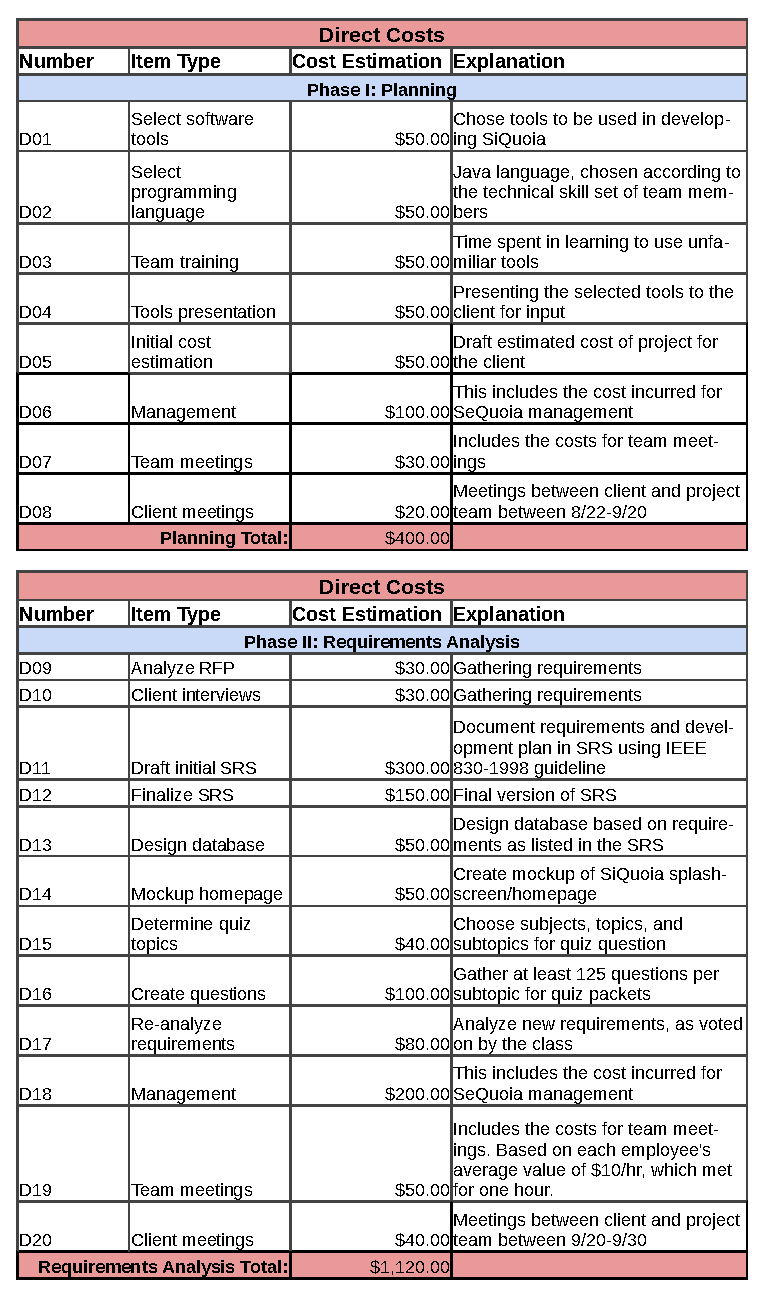
\includegraphics[width=0.7\textwidth]{chart0}
\newpage
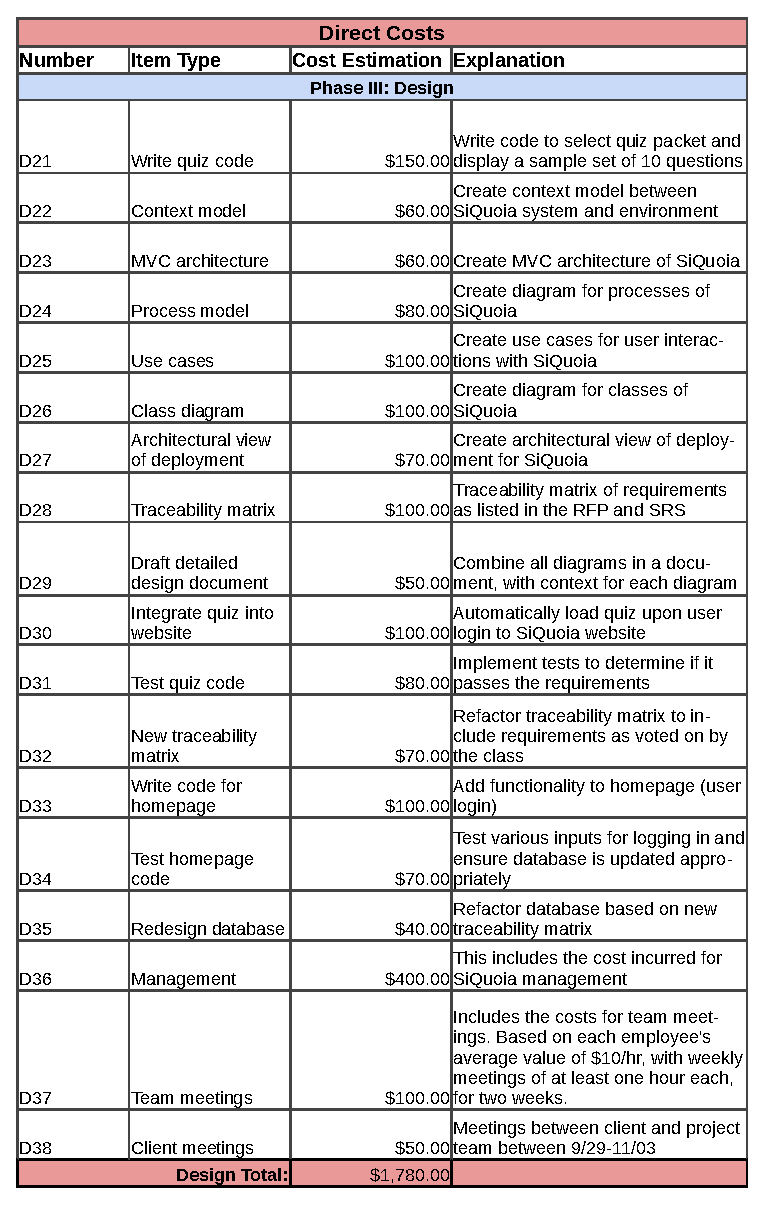
\includegraphics[width=0.7\textwidth]{chart1}
\newpage
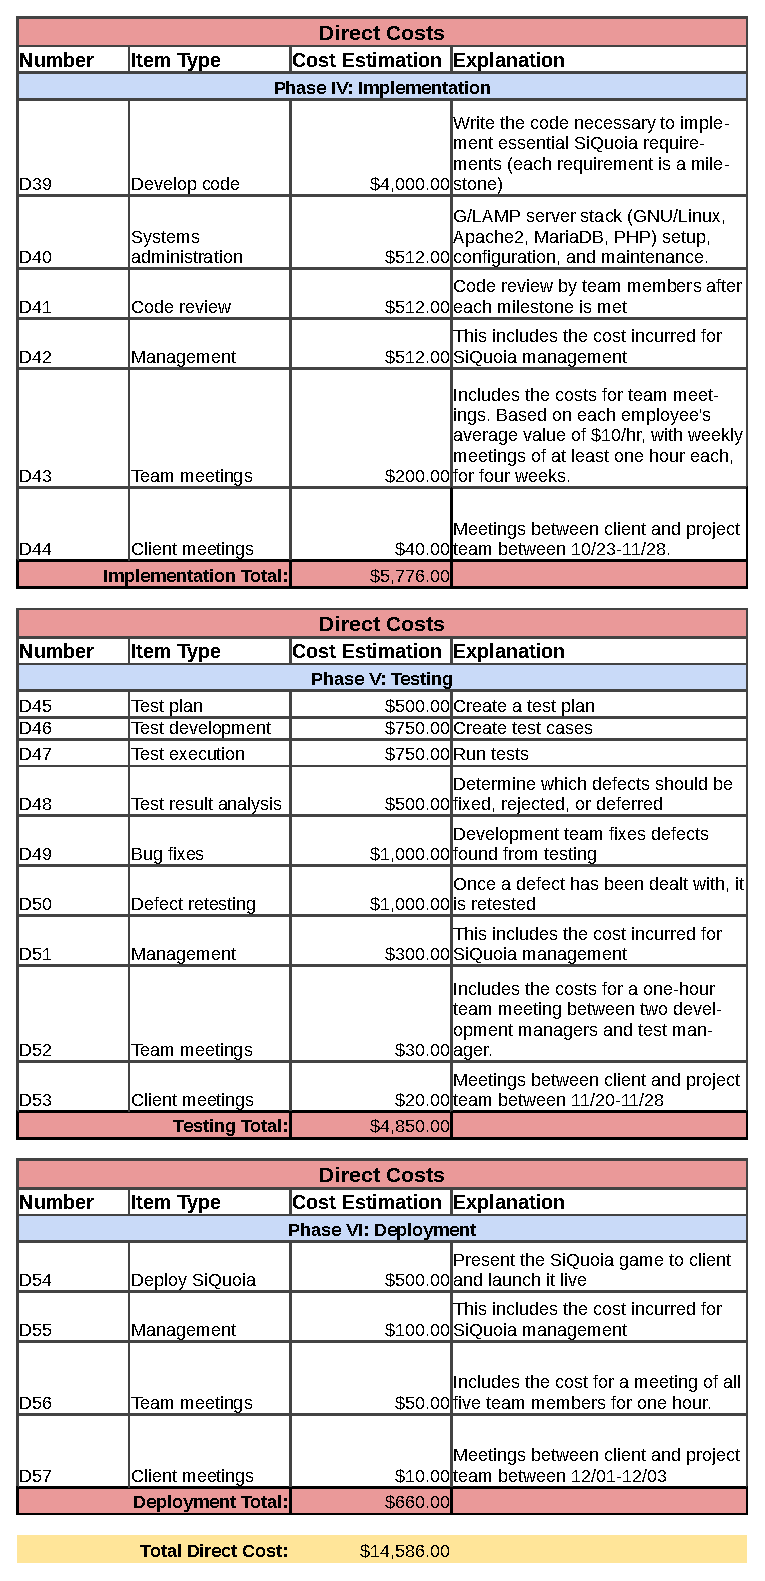
\includegraphics[width=0.66\textwidth]{chart2}
\newpage
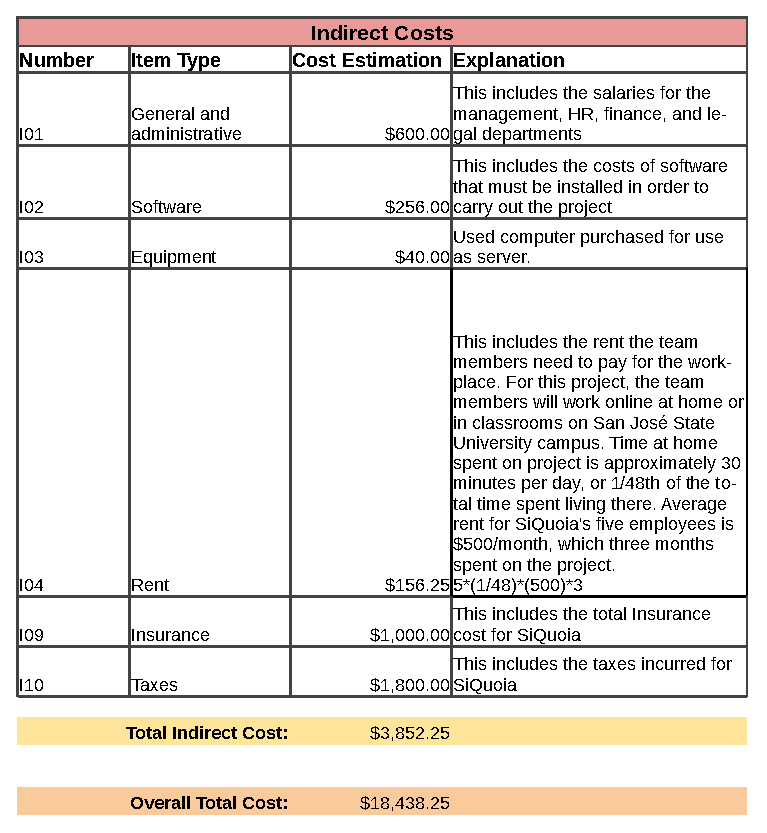
\includegraphics[width=0.7\textwidth]{chart3}
\end{center}

%\begin{thebibliography}{1}

%\bibitem{IEEEhowto:kopka}
%H.~Kopka and P.~W. Daly, \emph{A Guide to \LaTeX}, 3rd~ed.\hskip 1em plus
%  0.5em minus 0.4em\relax Harlow, England: Addison-Wesley, 1999.

%\end{thebibliography}


\end{document}


